\documentclass[10pt]{article}
\usepackage[margin=0.85in]{geometry}
\usepackage{amsmath,amssymb,booktabs,graphicx,caption}
\usepackage[hidelinks]{hyperref}
\captionsetup{font=small}
\setlength{\tabcolsep}{4pt}

\title{The $J_1$--$J_2$ model on $4\times L_x$ cylinders:\\ inputs, trial states, costs and crossover}
\author{Data report for the filter-pipeline paper}
\date{\today}

\begin{document}
\maketitle

\noindent This report collects every two-dimensional result produced for the paper. All tables and figures are
generated by \texttt{sbpipe\_study/report2d/make\_report2d.py} from \texttt{sbpipe\_study/results/*.json}
(\texttt{ext\_inputs2d.json}, \texttt{cache2d/}, \texttt{ext\_regime\_cyl*.json}, \texttt{emp\_regime.json},
\texttt{emp\_frontier.json}). Nothing in it is typed by hand.

\section{Model and pipeline settings}

\begin{equation}
H=J_1\sum_{\langle ij\rangle}\mathbf S_i\cdot\mathbf S_j+J_2\sum_{\langle\langle ij\rangle\rangle}\mathbf S_i\cdot\mathbf S_j,
\qquad J_1=1,
\end{equation}
on an $L_x\times4$ square lattice, periodic around the four-site circumference and open along $L_x=3,4,6,8,12$
($N=12$--48 qubits), at $J_2=0$ and $0.3$. Site $(x,y)$ is qubit $4x+y$, so the MPS runs up each column in
turn (a snake path). $J_2=0.5$ is left out because ED on $4\times4$ shows that its lowest excitation is not the
triplet, while the pipeline takes $E_1$ as the lowest $S^z=1$ state.

\begin{itemize}
\item \textbf{Energies.} DMRG (quimb) with reference bond dimensions $\chi=16,\dots,256$. $E_0$ and $E_1$ (the
lowest $S^z=1$ state) are taken from $\chi=256$, with the error estimated from the last change in $\chi$. The
spectral upper bound is Weyl's. ED is run for $4\times3$ and $4\times4$.
\item \textbf{Trial states.} Variational MPS at $\chi=2,\dots,64$. The overlap $\gamma=|\langle E_0|\psi_\chi\rangle|^2$
is measured against the $\chi=256$ reference (or ED). Each trial is costed as a staircase of
quantum-Shannon-decomposed unitaries.
\item \textbf{Filter.} QETU (Chebyshev) or the dyadic/optimized cosine filters, second-order Strang steps,
CNOT counts from Pauli-gadget ladders. \emph{Certified} costs come from the pipeline's a-priori
bound. \emph{Empirical} costs use the two laws measured on exact spectra for $N\le16$ (675 cases): the
smallest working degree is $d\,\Delta\simeq(2/\pi)\cosh^{-1}(1/\eta)$ with $\eta^2=\gamma\epsilon/(1-\gamma)$, and one
Strang step per query suffices.
\end{itemize}

\section{Energies and gaps}

\begin{table}[h]
\centering\small
\caption{Inputs per cylinder. $E_0$, $E_1$ from DMRG at $\chi\le256$; the errors are the pipeline inputs.
$E_{\max}$ is the Weyl upper bound, ``time'' is the wall-clock DMRG time in hours, and the last column gives
$|E^{\rm DMRG}-E^{\rm ED}|$ for $E_0$ and $E_1$ where ED is available.}
\begin{tabular}{lrrrrrrrrrc}
\toprule
system & $N$ & $J_2$ & $E_0$ & $E_1$ & gap & $\delta E_0$ & $\delta E_1$ & $E_{\max}$ & time [h] & ED check \\
\midrule
$4\times3$ & 12 & 0 & -7.530137 & -6.871724 & 0.6584 & $1.0\times10^{-10}$ & $1.0\times10^{-10}$ & 5.0 & 0.00 & $2\times10^{-14}$ / $4\times10^{-14}$ \\
$4\times4$ & 16 & 0 & -10.264290 & -9.688511 & 0.5758 & $1.3\times10^{-6}$ & $2.2\times10^{-6}$ & 7.0 & 0.12 & $2\times10^{-14}$ / $9\times10^{-12}$ \\
$4\times6$ & 24 & 0 & -15.728450 & -15.255513 & 0.4729 & $2.3\times10^{-5}$ & $3.4\times10^{-5}$ & 11.0 & 1.41 & -- \\
$4\times8$ & 32 & 0 & -21.194186 & -20.779712 & 0.4145 & $6.3\times10^{-5}$ & $1.0\times10^{-4}$ & 15.0 & 3.11 & -- \\
$4\times12$ & 48 & 0 & -32.126439 & -31.775997 & 0.3504 & $1.9\times10^{-4}$ & $3.4\times10^{-4}$ & 23.0 & 6.29 & -- \\
$4\times3$ & 12 & 0.3 & -6.598094 & -5.869734 & 0.7284 & $1.0\times10^{-10}$ & $1.0\times10^{-10}$ & 6.2 & 0.00 & $2\times10^{-14}$ / $8\times10^{-15}$ \\
$4\times4$ & 16 & 0.3 & -8.888556 & -8.220986 & 0.6676 & $3.4\times10^{-6}$ & $2.2\times10^{-6}$ & 8.8 & 0.12 & $8\times10^{-14}$ / $1\times10^{-11}$ \\
$4\times6$ & 24 & 0.3 & -13.465810 & -12.874454 & 0.5914 & $2.8\times10^{-5}$ & $7.8\times10^{-5}$ & 14.0 & 1.46 & -- \\
$4\times8$ & 32 & 0.3 & -18.043497 & -17.492736 & 0.5508 & $5.9\times10^{-5}$ & $2.1\times10^{-4}$ & 19.2 & 2.56 & -- \\
$4\times12$ & 48 & 0.3 & -27.198944 & -26.688843 & 0.5101 & $1.2\times10^{-4}$ & $5.4\times10^{-4}$ & 29.6 & 6.11 & -- \\
\bottomrule
\end{tabular}
\end{table}

The triplet gap closes slowly with $L_x$: from 0.66 to 0.35 at $J_2=0$ and from 0.73 to 0.51 at $J_2=0.3$
(Fig.~\ref{fig:inputs}c). Frustration opens the finite-size gap here. Because the Weyl bound grows as $N$, the
scaled gap $\Delta=g/W$ that sets the filter degree falls roughly as $1/N$. The DMRG energy errors grow
from $10^{-10}$ ($4\times3$, exact at $\chi=64$) to $2$--$5\times10^{-4}$ at $4\times12$. Where ED exists, DMRG matches it to
$10^{-11}$ or better.

\begin{table}[h]
\centering\small
\caption{DMRG convergence of $E_0$: $|E_0(\chi)-E_0(256)|$.}
\begin{tabular}{lrccccc}
\toprule
system & $J_2$ & $\chi=16$ & 32 & 64 & 128 & 256 \\
\midrule
$4\times3$ & 0 & $2\times10^{-2}$ & $7\times10^{-4}$ & $8\times10^{-15}$ & $1\times10^{-14}$ & ref \\
$4\times4$ & 0 & $5\times10^{-2}$ & $4\times10^{-3}$ & $1\times10^{-4}$ & $1\times10^{-6}$ & ref \\
$4\times6$ & 0 & $9\times10^{-2}$ & $1\times10^{-2}$ & $5\times10^{-4}$ & $2\times10^{-5}$ & ref \\
$4\times8$ & 0 & $1\times10^{-1}$ & $2\times10^{-2}$ & $1\times10^{-3}$ & $6\times10^{-5}$ & ref \\
$4\times12$ & 0 & $2\times10^{-1}$ & $4\times10^{-2}$ & $2\times10^{-3}$ & $2\times10^{-4}$ & ref \\
$4\times3$ & 0.3 & $1\times10^{-2}$ & $3\times10^{-4}$ & $6\times10^{-15}$ & $3\times10^{-15}$ & ref \\
$4\times4$ & 0.3 & $3\times10^{-2}$ & $2\times10^{-3}$ & $1\times10^{-4}$ & $3\times10^{-6}$ & ref \\
$4\times6$ & 0.3 & $5\times10^{-2}$ & $6\times10^{-3}$ & $5\times10^{-4}$ & $3\times10^{-5}$ & ref \\
$4\times8$ & 0.3 & $8\times10^{-2}$ & $1\times10^{-2}$ & $9\times10^{-4}$ & $6\times10^{-5}$ & ref \\
$4\times12$ & 0.3 & $1\times10^{-1}$ & $2\times10^{-2}$ & $2\times10^{-3}$ & $1\times10^{-4}$ & ref \\
\bottomrule
\end{tabular}
\end{table}

\begin{figure}[h]
\centering
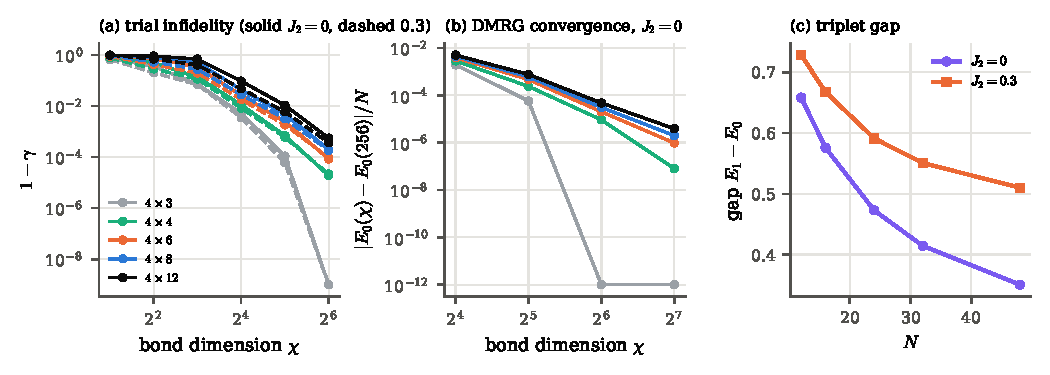
\includegraphics[width=\textwidth]{figs/fig_inputs.pdf}
\caption{(a) Trial infidelity $1-\gamma$ versus bond dimension for every cylinder (solid $J_2=0$, dashed $J_2=0.3$).
(b) DMRG energy convergence per site. (c) Triplet gap versus $N$.}
\label{fig:inputs}
\end{figure}

\section{Trial states: overlap and circuit cost}

\begin{table}[h]
\centering\small
\caption{Trial infidelity $1-\gamma$ of the variational MPS. Values at the $10^{-4}$ level and below for
$L_x\ge8$ are limited by the accuracy of the $\chi=256$ reference.}
\begin{tabular}{lrcccccc}
\toprule
system & $J_2$ & $\chi=2$ & 4 & 8 & 16 & 32 & 64 \\
\midrule
$4\times3$ & 0 & $7.3\times10^{-1}$ & $3.7\times10^{-1}$ & $7.0\times10^{-2}$ & $5.2\times10^{-3}$ & $1.1\times10^{-4}$ & $<10^{-9}$ \\
$4\times4$ & 0 & $8.1\times10^{-1}$ & $5.1\times10^{-1}$ & $1.3\times10^{-1}$ & $1.1\times10^{-2}$ & $7.0\times10^{-4}$ & $1.9\times10^{-5}$ \\
$4\times6$ & 0 & $9.0\times10^{-1}$ & $7.3\times10^{-1}$ & $3.4\times10^{-1}$ & $2.6\times10^{-2}$ & $2.4\times10^{-3}$ & $8.5\times10^{-5}$ \\
$4\times8$ & 0 & $9.5\times10^{-1}$ & $8.1\times10^{-1}$ & $5.2\times10^{-1}$ & $4.3\times10^{-2}$ & $4.8\times10^{-3}$ & $2.0\times10^{-4}$ \\
$4\times12$ & 0 & $9.8\times10^{-1}$ & $9.1\times10^{-1}$ & $6.9\times10^{-1}$ & $9.5\times10^{-2}$ & $1.1\times10^{-2}$ & $5.5\times10^{-4}$ \\
$4\times3$ & 0.3 & $6.6\times10^{-1}$ & $2.0\times10^{-1}$ & $6.9\times10^{-2}$ & $3.6\times10^{-3}$ & $6.1\times10^{-5}$ & $<10^{-9}$ \\
$4\times4$ & 0.3 & $7.8\times10^{-1}$ & $2.9\times10^{-1}$ & $1.1\times10^{-1}$ & $8.3\times10^{-3}$ & $6.0\times10^{-4}$ & $2.2\times10^{-5}$ \\
$4\times6$ & 0.3 & $8.9\times10^{-1}$ & $4.2\times10^{-1}$ & $2.0\times10^{-1}$ & $1.8\times10^{-2}$ & $1.8\times10^{-3}$ & $9.6\times10^{-5}$ \\
$4\times8$ & 0.3 & $9.5\times10^{-1}$ & $5.3\times10^{-1}$ & $2.8\times10^{-1}$ & $2.8\times10^{-2}$ & $3.2\times10^{-3}$ & $1.8\times10^{-4}$ \\
$4\times12$ & 0.3 & $9.9\times10^{-1}$ & $7.0\times10^{-1}$ & $4.1\times10^{-1}$ & $4.8\times10^{-2}$ & $6.0\times10^{-3}$ & $3.7\times10^{-4}$ \\
\bottomrule
\end{tabular}
\end{table}

\begin{table}[h]
\centering\small
\caption{CNOTs of the MPS preparation circuit (independent of $J_2$).}
\begin{tabular}{lcccccc}
\toprule
system & $\chi=2$ & 4 & 8 & 16 & 32 & 64 \\
\midrule
$4\times3$ & $3.3\times10^{1}$ & $2.0\times10^{2}$ & $9.0\times10^{2}$ & $3.6\times10^{3}$ & $1.3\times10^{4}$ & $4.6\times10^{4}$ \\
$4\times4$ & $4.5\times10^{1}$ & $2.8\times10^{2}$ & $1.3\times10^{3}$ & $5.3\times10^{3}$ & $2.1\times10^{4}$ & $7.7\times10^{4}$ \\
$4\times6$ & $6.9\times10^{1}$ & $4.4\times10^{2}$ & $2.1\times10^{3}$ & $8.9\times10^{3}$ & $3.5\times10^{4}$ & $1.4\times10^{5}$ \\
$4\times8$ & $9.3\times10^{1}$ & $6.0\times10^{2}$ & $2.9\times10^{3}$ & $1.2\times10^{4}$ & $5.0\times10^{4}$ & $2.0\times10^{5}$ \\
$4\times12$ & $1.4\times10^{2}$ & $9.2\times10^{2}$ & $4.5\times10^{3}$ & $2.0\times10^{4}$ & $8.0\times10^{4}$ & $3.2\times10^{5}$ \\
\bottomrule
\end{tabular}
\end{table}

Compared with the chain, the snake MPS converges much more slowly in $\chi$. The 48-site chain reaches
$1-\gamma\le10^{-2}$ at $\chi=8$; the $4\times12$ cylinder needs $\chi=32$ for the same, and $\chi=64$ leaves
$5.5\times10^{-4}$ ($J_2=0$). The trial cost grows as $\chi^2N$, so each doubling of $\chi$ costs about $4\times$.
That combination (slow convergence, quadratic cost) is what opens room for the filter.

\section{Cheapest route to a fixed target}

Table~\ref{tab:regime} compares three routes at $\epsilon=10^{-2},10^{-3},10^{-4}$:
\begin{itemize}
\item the cheapest MPS that meets $1-\gamma\le\epsilon$ on its own;
\item the cheapest certified filtered plan (any $\chi$; dyadic, optimized or QETU);
\item the cheapest empirical filtered plan (QETU at the degree law, one step per query).
\end{itemize}
Filtered costs are expected CNOTs per success, including the trial circuit on every attempt.

\begin{table}[h]
\centering\footnotesize
\caption{CNOTs (bond dimension in parentheses). M: MPS alone. C: certified filter. E: empirical filter.
``--'': no $\chi\le64$ route.}
\label{tab:regime}
\resizebox{\textwidth}{!}{%
\begin{tabular}{lr ccc ccc ccc}
\toprule
 & & \multicolumn{3}{c}{$\epsilon=10^{-2}$} & \multicolumn{3}{c}{$\epsilon=10^{-3}$} & \multicolumn{3}{c}{$\epsilon=10^{-4}$}\\
\cmidrule(lr){3-5}\cmidrule(lr){6-8}\cmidrule(lr){9-11}
system & $J_2$ & M & C & E & M & C & E & M & C & E \\
\midrule
$4\times3$ & 0 & $3.6\times10^{3}$ (16) & $4.9\times10^{4}$ (8) & $1.2\times10^{4}$ (8) & $1.3\times10^{4}$ (32) & $7.4\times10^{4}$ (16) & $1.2\times10^{4}$ (16) & $4.6\times10^{4}$ (64) & $6.5\times10^{4}$ (32) & $1.5\times10^{4}$ (32) \\
$4\times4$ & 0 & $2.1\times10^{4}$ (32) & $6.3\times10^{4}$ (16) & $1.1\times10^{4}$ (16) & $2.1\times10^{4}$ (32) & $2.7\times10^{5}$ (16) & $3.0\times10^{4}$ (16) & $7.7\times10^{4}$ (64) & $4.0\times10^{5}$ (32) & $4.2\times10^{4}$ (32) \\
$4\times6$ & 0 & $3.5\times10^{4}$ (32) & $2.6\times10^{5}$ (16) & $5.2\times10^{4}$ (16) & $1.4\times10^{5}$ (64) & $4.3\times10^{5}$ (32) & $7.6\times10^{4}$ (32) & $1.4\times10^{5}$ (64) & $1.6\times10^{6}$ (32) & $1.2\times10^{5}$ (32) \\
$4\times8$ & 0 & $5.0\times10^{4}$ (32) & $6.9\times10^{5}$ (16) & $1.3\times10^{5}$ (16) & $2.0\times10^{5}$ (64) & $1.2\times10^{6}$ (32) & $1.7\times10^{5}$ (32) & -- & $1.4\times10^{6}$ (64) & $2.6\times10^{5}$ (32) \\
$4\times12$ & 0 & $3.2\times10^{5}$ (64) & $7.5\times10^{5}$ (32) & $1.4\times10^{5}$ (32) & $3.2\times10^{5}$ (64) & $3.9\times10^{6}$ (32) & $5.0\times10^{5}$ (32) & -- & $5.7\times10^{6}$ (64) & $6.6\times10^{5}$ (64) \\
$4\times3$ & 0.3 & $3.6\times10^{3}$ (16) & $1.2\times10^{5}$ (8) & $1.9\times10^{4}$ (8) & $1.3\times10^{4}$ (32) & $1.3\times10^{5}$ (16) & $1.6\times10^{4}$ (16) & $1.3\times10^{4}$ (32) & $4.5\times10^{5}$ (16) & $2.8\times10^{4}$ (16) \\
$4\times4$ & 0.3 & $5.3\times10^{3}$ (16) & $4.8\times10^{5}$ (8) & $4.9\times10^{4}$ (8) & $2.1\times10^{4}$ (32) & $5.6\times10^{5}$ (16) & $4.3\times10^{4}$ (16) & $7.7\times10^{4}$ (64) & $9.1\times10^{5}$ (32) & $5.3\times10^{4}$ (32) \\
$4\times6$ & 0.3 & $3.5\times10^{4}$ (32) & $5.0\times10^{5}$ (16) & $6.2\times10^{4}$ (16) & $1.4\times10^{5}$ (64) & $8.2\times10^{5}$ (32) & $8.8\times10^{4}$ (32) & $1.4\times10^{5}$ (64) & $3.4\times10^{6}$ (32) & $1.6\times10^{5}$ (32) \\
$4\times8$ & 0.3 & $5.0\times10^{4}$ (32) & $1.2\times10^{6}$ (16) & $1.6\times10^{5}$ (16) & $2.0\times10^{5}$ (64) & $2.0\times10^{6}$ (32) & $2.0\times10^{5}$ (32) & -- & $2.7\times10^{6}$ (64) & $3.0\times10^{5}$ (64) \\
$4\times12$ & 0.3 & $8.0\times10^{4}$ (32) & $3.3\times10^{6}$ (16) & $4.9\times10^{5}$ (16) & $3.2\times10^{5}$ (64) & $5.9\times10^{6}$ (32) & $5.6\times10^{5}$ (32) & -- & $8.5\times10^{6}$ (64) & $7.1\times10^{5}$ (64) \\
\bottomrule
\end{tabular}}
\end{table}

\paragraph{Certified.} The certified filter never beats a compiled MPS that reaches the target, usually missing by
one to two orders of magnitude. It is the only route at $\epsilon=10^{-4}$ on $4\times8$ and $4\times12$, where no
$\chi\le64$ trial suffices. Its excess comes almost entirely from the Trotter bound, which asks for about
16 steps per query where one is enough.

\paragraph{Empirical.} With the measured filter cost the comparison depends on where the target falls on the
MPS staircase. The empirical filter wins whenever the target lies just beyond what the current $\chi$ reaches, so that
the MPS would need the next doubling: for example $4\times4$ at $10^{-2}$ and $10^{-4}$, $4\times6$ and $4\times8$ at
$10^{-3}$, and $4\times12$ at $10^{-2}$ ($J_2=0$). Otherwise it loses, by up to $6\times$ (e.g. $4\times12$, $J_2=0.3$,
$10^{-2}$, where $\chi=32$ already suffices). It is the only route at $10^{-4}$ on $4\times8$ and $4\times12$.

\paragraph{Check of the empirical laws.} For $4\times3$ and $4\times4$ (and the 16-site chain) the trial
state vectors are available. There we ran the actual QETU circuit, one Strang step per query, at the degree
the law predicts. In 48 of 48 cases it met the target at exactly that degree
(Table~\ref{tab:sim}).

\begin{table}[h]
\centering\small
\caption{State-vector simulation of the empirical filter on cylinders: predicted degree, degree that
reached $\epsilon$ with one Strang step per query, measured infidelity and success probability.}
\label{tab:sim}
\begin{tabular}{lrrrcrrcc}
\toprule
system & $J_2$ & $\chi$ & $\gamma$ & $\epsilon$ & $d$ (law) & $d$ (sim) & $1-F$ & $p$ \\
\midrule
$4\times3$ & 0 & 2 & 0.2697 & $1\times10^{-2}$ & 44 & 44 & $4.5\times10^{-3}$ & 0.271 \\
$4\times3$ & 0.3 & 2 & 0.3391 & $1\times10^{-2}$ & 38 & 38 & $5.0\times10^{-3}$ & 0.340 \\
$4\times3$ & 0 & 2 & 0.2697 & $1\times10^{-3}$ & 58 & 58 & $3.9\times10^{-4}$ & 0.270 \\
$4\times3$ & 0.3 & 2 & 0.3391 & $1\times10^{-3}$ & 52 & 52 & $3.6\times10^{-4}$ & 0.338 \\
$4\times3$ & 0 & 2 & 0.2697 & $1\times10^{-4}$ & 72 & 72 & $4.9\times10^{-5}$ & 0.269 \\
$4\times3$ & 0.3 & 2 & 0.3391 & $1\times10^{-4}$ & 64 & 64 & $3.4\times10^{-5}$ & 0.338 \\
$4\times3$ & 0 & 4 & 0.6333 & $1\times10^{-2}$ & 34 & 34 & $5.0\times10^{-3}$ & 0.638 \\
$4\times3$ & 0.3 & 4 & 0.7978 & $1\times10^{-2}$ & 26 & 26 & $2.6\times10^{-3}$ & 0.800 \\
$4\times3$ & 0 & 4 & 0.6333 & $1\times10^{-3}$ & 48 & 48 & $4.5\times10^{-4}$ & 0.634 \\
$4\times3$ & 0.3 & 4 & 0.7978 & $1\times10^{-3}$ & 40 & 40 & $5.7\times10^{-4}$ & 0.798 \\
$4\times3$ & 0 & 4 & 0.6333 & $1\times10^{-4}$ & 62 & 62 & $9.0\times10^{-5}$ & 0.634 \\
$4\times3$ & 0.3 & 4 & 0.7978 & $1\times10^{-4}$ & 52 & 52 & $3.1\times10^{-5}$ & 0.797 \\
$4\times3$ & 0 & 8 & 0.9300 & $1\times10^{-2}$ & 22 & 22 & $5.7\times10^{-3}$ & 0.936 \\
$4\times3$ & 0.3 & 8 & 0.9309 & $1\times10^{-2}$ & 20 & 20 & $6.0\times10^{-3}$ & 0.936 \\
$4\times3$ & 0 & 8 & 0.9300 & $1\times10^{-3}$ & 36 & 36 & $3.2\times10^{-4}$ & 0.931 \\
$4\times3$ & 0.3 & 8 & 0.9309 & $1\times10^{-3}$ & 32 & 32 & $5.2\times10^{-4}$ & 0.931 \\
$4\times3$ & 0 & 8 & 0.9300 & $1\times10^{-4}$ & 50 & 50 & $3.2\times10^{-5}$ & 0.930 \\
$4\times3$ & 0.3 & 8 & 0.9309 & $1\times10^{-4}$ & 46 & 46 & $3.9\times10^{-5}$ & 0.930 \\
$4\times3$ & 0 & 16 & 0.9948 & $1\times10^{-3}$ & 18 & 18 & $5.2\times10^{-4}$ & 0.995 \\
$4\times3$ & 0.3 & 16 & 0.9964 & $1\times10^{-3}$ & 14 & 14 & $3.0\times10^{-4}$ & 0.996 \\
$4\times3$ & 0 & 16 & 0.9948 & $1\times10^{-4}$ & 34 & 34 & $4.1\times10^{-5}$ & 0.994 \\
$4\times3$ & 0.3 & 16 & 0.9964 & $1\times10^{-4}$ & 28 & 28 & $5.5\times10^{-5}$ & 0.995 \\
$4\times3$ & 0 & 32 & 0.9999 & $1\times10^{-4}$ & 4 & 4 & $9.2\times10^{-5}$ & 1.000 \\
$4\times4$ & 0 & 2 & 0.1891 & $1\times10^{-2}$ & 72 & 72 & $4.9\times10^{-3}$ & 0.190 \\
$4\times4$ & 0.3 & 2 & 0.2249 & $1\times10^{-2}$ & 62 & 62 & $4.5\times10^{-3}$ & 0.225 \\
$4\times4$ & 0 & 2 & 0.1891 & $1\times10^{-3}$ & 94 & 94 & $4.6\times10^{-4}$ & 0.189 \\
$4\times4$ & 0.3 & 2 & 0.2249 & $1\times10^{-3}$ & 82 & 82 & $3.9\times10^{-4}$ & 0.224 \\
$4\times4$ & 0 & 2 & 0.1891 & $1\times10^{-4}$ & 116 & 116 & $5.0\times10^{-5}$ & 0.189 \\
$4\times4$ & 0.3 & 2 & 0.2249 & $1\times10^{-4}$ & 100 & 100 & $4.1\times10^{-5}$ & 0.224 \\
$4\times4$ & 0 & 4 & 0.4946 & $1\times10^{-2}$ & 58 & 58 & $5.4\times10^{-3}$ & 0.498 \\
$4\times4$ & 0.3 & 4 & 0.7148 & $1\times10^{-2}$ & 44 & 44 & $2.7\times10^{-3}$ & 0.716 \\
$4\times4$ & 0 & 4 & 0.4946 & $1\times10^{-3}$ & 80 & 80 & $4.2\times10^{-4}$ & 0.495 \\
$4\times4$ & 0.3 & 4 & 0.7148 & $1\times10^{-3}$ & 64 & 64 & $3.0\times10^{-4}$ & 0.715 \\
$4\times4$ & 0 & 4 & 0.4946 & $1\times10^{-4}$ & 102 & 102 & $4.2\times10^{-5}$ & 0.495 \\
$4\times4$ & 0.3 & 4 & 0.7148 & $1\times10^{-4}$ & 82 & 82 & $6.4\times10^{-5}$ & 0.714 \\
$4\times4$ & 0 & 8 & 0.8660 & $1\times10^{-2}$ & 40 & 40 & $5.5\times10^{-3}$ & 0.871 \\
$4\times4$ & 0.3 & 8 & 0.8852 & $1\times10^{-2}$ & 34 & 34 & $5.6\times10^{-3}$ & 0.890 \\
$4\times4$ & 0 & 8 & 0.8660 & $1\times10^{-3}$ & 62 & 62 & $6.2\times10^{-4}$ & 0.867 \\
$4\times4$ & 0.3 & 8 & 0.8852 & $1\times10^{-3}$ & 54 & 54 & $5.6\times10^{-4}$ & 0.885 \\
$4\times4$ & 0 & 8 & 0.8660 & $1\times10^{-4}$ & 84 & 84 & $7.0\times10^{-5}$ & 0.866 \\
$4\times4$ & 0.3 & 8 & 0.8852 & $1\times10^{-4}$ & 74 & 74 & $4.0\times10^{-5}$ & 0.884 \\
$4\times4$ & 0 & 16 & 0.9889 & $1\times10^{-2}$ & 8 & 8 & $3.9\times10^{-3}$ & 0.993 \\
$4\times4$ & 0 & 16 & 0.9889 & $1\times10^{-3}$ & 36 & 36 & $5.6\times10^{-4}$ & 0.989 \\
$4\times4$ & 0.3 & 16 & 0.9917 & $1\times10^{-3}$ & 30 & 30 & $5.7\times10^{-4}$ & 0.992 \\
$4\times4$ & 0 & 16 & 0.9889 & $1\times10^{-4}$ & 60 & 60 & $4.3\times10^{-5}$ & 0.988 \\
$4\times4$ & 0.3 & 16 & 0.9917 & $1\times10^{-4}$ & 50 & 50 & $5.3\times10^{-5}$ & 0.991 \\
$4\times4$ & 0 & 32 & 0.9993 & $1\times10^{-4}$ & 32 & 32 & $7.0\times10^{-5}$ & 0.999 \\
$4\times4$ & 0.3 & 32 & 0.9994 & $1\times10^{-4}$ & 26 & 26 & $5.1\times10^{-5}$ & 0.999 \\
\bottomrule
\end{tabular}
\end{table}

\section{Cost per accuracy and the crossover}

For a continuous view we compute the cheapest cost to reach every infidelity between $10^{-1}$ and $10^{-7}$
(Fig.~\ref{fig:cross}):
\begin{itemize}
\item MPS alone: the cheapest $\chi$ with $1-\gamma\le\epsilon$, a staircase in $\epsilon$;
\item the empirical filter: minimized over the trial $\chi$;
\item the certified filter: at the three targets above.
\end{itemize}

\begin{figure}[h]
\centering
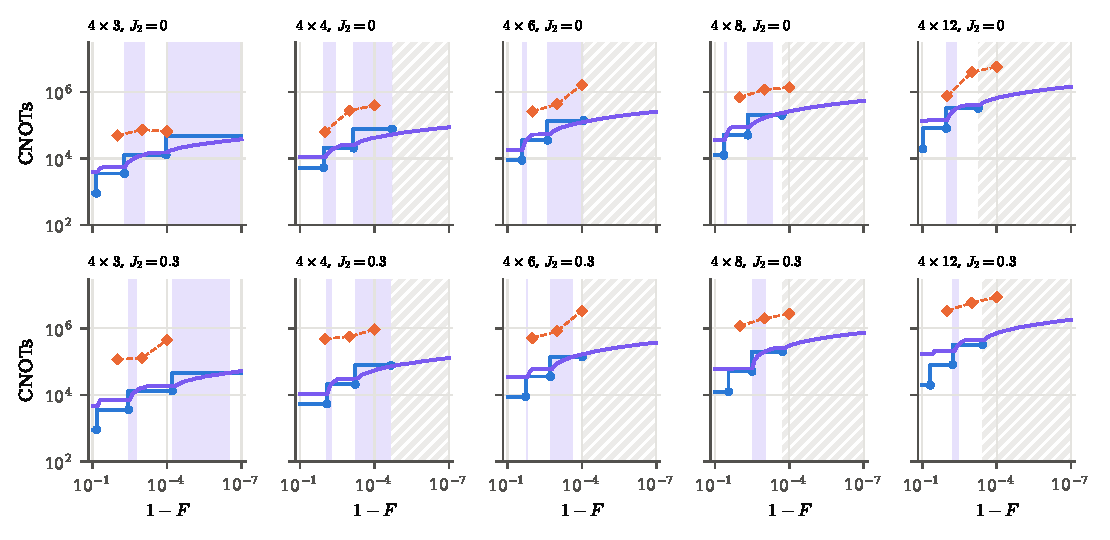
\includegraphics[width=\textwidth]{figs/fig_crossover2d.pdf}
\caption{Cheapest CNOTs to reach infidelity $1-F$ (accuracy increases to the right). Blue: MPS alone (dots are the
$\chi=2,\dots,64$ trials). Purple: MPS + filter, empirical. Orange diamonds: MPS + filter, certified. Purple
shading: the empirical filter is cheaper. Grey hatching: no MPS with $\chi\le64$ reaches that accuracy.}
\label{fig:cross}
\end{figure}

\begin{table}[h]
\centering\small
\caption{Accuracy windows in which the empirical filter is cheaper than any MPS that meets the target alone
(largest saving in parentheses; windows narrower than a factor 1.5 in $1-F$ omitted), and the accuracy
beyond which no $\chi\le64$ MPS suffices.}
\begin{tabular}{lrlc}
\toprule
system & $J_2$ & filter cheaper for $1-F$ in & MPS ($\chi\le64$) limit \\
\midrule
$4\times3$ & 0 & $5\times10^{-3}$--$8\times10^{-4}$ ($2.4\times$); $1\times10^{-4}$--$1\times10^{-7}$ ($3.1\times$) & -- \\
$4\times4$ & 0 & $1\times10^{-2}$--$4\times10^{-3}$ ($1.9\times$); $7\times10^{-4}$--$2\times10^{-5}$ ($3.0\times$) & $2\times10^{-5}$ \\
$4\times6$ & 0 & $2\times10^{-3}$--$9\times10^{-5}$ ($2.6\times$) & $8\times10^{-5}$ \\
$4\times8$ & 0 & $5\times10^{-3}$--$5\times10^{-4}$ ($2.3\times$) & $2\times10^{-4}$ \\
$4\times12$ & 0 & $1\times10^{-2}$--$4\times10^{-3}$ ($2.3\times$) & $5\times10^{-4}$ \\
$4\times3$ & 0.3 & $4\times10^{-3}$--$2\times10^{-3}$ ($1.9\times$); $6\times10^{-5}$--$3\times10^{-7}$ ($2.5\times$) & -- \\
$4\times4$ & 0.3 & $6\times10^{-4}$--$2\times10^{-5}$ ($2.5\times$) & $2\times10^{-5}$ \\
$4\times6$ & 0.3 & $2\times10^{-3}$--$2\times10^{-4}$ ($2.3\times$) & $1\times10^{-4}$ \\
$4\times8$ & 0.3 & $3\times10^{-3}$--$1\times10^{-3}$ ($3.2\times$) & $2\times10^{-4}$ \\
$4\times12$ & 0.3 & $6\times10^{-3}$--$3\times10^{-3}$ ($1.5\times$) & $4\times10^{-4}$ \\
\bottomrule
\end{tabular}
\end{table}

\paragraph{Reading the crossover.} On every cylinder the empirical filter wins in the accuracy window just
before the MPS needs its next doubling of $\chi$: a short filter on the current $\chi$ is cheaper than a
$4\times$ larger trial circuit. The saving in that window is a factor of 2--3. Two trends follow from the inputs:
\begin{itemize}
\item The window moves to looser accuracy as the cylinder grows (from around $10^{-4}$ at $4\times4$ to around
$10^{-2}$ at $4\times12$). Each $\chi$ buys less overlap on a longer cylinder, while the filter degree depends on
the overlap only logarithmically.
\item Beyond the MPS limit ($2\times10^{-5}$ at $4\times4$, $5\times10^{-4}$ at $4\times12$) the filter is the only
route in our data. A $\chi=128$ trial would cost about $4\times$ the $\chi=64$ one, roughly $1.3\times10^{6}$ CNOTs at
$4\times12$, about what the empirical filter needs for $1-F=10^{-6}$ and more than it needs at any looser target, even if such a trial reached that accuracy.
\end{itemize}
The chain has no such crossover (see the regime section of the paper): its MPS overlap converges fast enough in $\chi$ that the next
doubling is always the cheaper option.

\section{Caveats}
\begin{itemize}
\item The empirical filter cost rests on two laws measured for $N\le16$ (chain and the two small cylinders).
They held in every case we could simulate, but beyond $N=16$ they are extrapolated, and they are not a
certificate. Only the certified curve carries a guarantee, and it does not cross the MPS.
\item Overlaps at the $10^{-4}$ level and below for $L_x\ge8$, and energy errors of $2$--$5\times10^{-4}$ at $4\times12$,
are limited by the $\chi=256$ DMRG reference. The MPS staircase is therefore uncertain at its tight end on
the larger cylinders.
\item ED confirms the triplet as the first excitation only for $4\times3$ and $4\times4$. For larger cylinders
this is an assumption.
\item Costs are CNOT counts with all-to-all connectivity. Trial circuits use a generic decomposition bound,
not compiled circuits. Repeat-until-success is assumed throughout.
\item Only width-4 cylinders were studied. Wider cylinders, where the snake MPS degrades faster, are the
natural next test of whether the crossover window widens.
\end{itemize}

\end{document}
